\documentclass[14pt,xcolor=pdftex,dvipsnames,table]{beamer}\usepackage[]{graphicx}\usepackage[]{color}
%% maxwidth is the original width if it is less than linewidth
%% otherwise use linewidth (to make sure the graphics do not exceed the margin)
\makeatletter
\def\maxwidth{ %
  \ifdim\Gin@nat@width>\linewidth
    \linewidth
  \else
    \Gin@nat@width
  \fi
}
\makeatother

\definecolor{fgcolor}{rgb}{0.345, 0.345, 0.345}
\newcommand{\hlnum}[1]{\textcolor[rgb]{0.686,0.059,0.569}{#1}}%
\newcommand{\hlstr}[1]{\textcolor[rgb]{0.192,0.494,0.8}{#1}}%
\newcommand{\hlcom}[1]{\textcolor[rgb]{0.678,0.584,0.686}{\textit{#1}}}%
\newcommand{\hlopt}[1]{\textcolor[rgb]{0,0,0}{#1}}%
\newcommand{\hlstd}[1]{\textcolor[rgb]{0.345,0.345,0.345}{#1}}%
\newcommand{\hlkwa}[1]{\textcolor[rgb]{0.161,0.373,0.58}{\textbf{#1}}}%
\newcommand{\hlkwb}[1]{\textcolor[rgb]{0.69,0.353,0.396}{#1}}%
\newcommand{\hlkwc}[1]{\textcolor[rgb]{0.333,0.667,0.333}{#1}}%
\newcommand{\hlkwd}[1]{\textcolor[rgb]{0.737,0.353,0.396}{\textbf{#1}}}%

\usepackage{framed}
\makeatletter
\newenvironment{kframe}{%
 \def\at@end@of@kframe{}%
 \ifinner\ifhmode%
  \def\at@end@of@kframe{\end{minipage}}%
  \begin{minipage}{\columnwidth}%
 \fi\fi%
 \def\FrameCommand##1{\hskip\@totalleftmargin \hskip-\fboxsep
 \colorbox{shadecolor}{##1}\hskip-\fboxsep
     % There is no \\@totalrightmargin, so:
     \hskip-\linewidth \hskip-\@totalleftmargin \hskip\columnwidth}%
 \MakeFramed {\advance\hsize-\width
   \@totalleftmargin\z@ \linewidth\hsize
   \@setminipage}}%
 {\par\unskip\endMakeFramed%
 \at@end@of@kframe}
\makeatother

\definecolor{shadecolor}{rgb}{.97, .97, .97}
\definecolor{messagecolor}{rgb}{0, 0, 0}
\definecolor{warningcolor}{rgb}{1, 0, 1}
\definecolor{errorcolor}{rgb}{1, 0, 0}
\newenvironment{knitrout}{}{} % an empty environment to be redefined in TeX

\usepackage{alltt}

% Specify theme
\usetheme{Madrid}
% See deic.uab.es/~iblanes/beamer_gallery/index_by_theme.html for other themes
\usepackage{caption}
\usepackage[comma, sort&compress]{natbib}
\usepackage{graphicx}
\usepackage{amsmath}
\bibliographystyle{agsm}
% Specify base color
\usecolortheme[named=OliveGreen]{structure}
% See http://goo.gl/p0Phn for other colors

% Specify other colors and options as required
\setbeamercolor{alerted text}{fg=Maroon}
\setbeamertemplate{items}[square]

% Title and author information
\title{Introduction to Regression}
\author{Rob Hayward}
\IfFileExists{upquote.sty}{\usepackage{upquote}}{}


\begin{document}

\begin{frame}
\titlepage
\end{frame}

\begin{frame}{Outline}
\tableofcontents
\end{frame}


\section{Modelling}
\begin{frame}{Model for securities}
Model security return.  You have thought about this already as it is an important component of 
\begin{itemize}[<+-| alert@+>]
\item  CAPM
\begin{itemize}
\item Beta is the relationship between securities returns and the market
\end{itemize}
\item Diversification
\begin{itemize}
\item Distinguish market risk and ideosyncratic risk
\end{itemize}
\item EMH
\begin{itemize}
\item What is the ideosyncratic or individual performance of the security?
\end{itemize}
\end{itemize}
\end{frame}



\begin{frame}{Modelling}
The model
\begin{block}{}
$y_t = \alpha + \beta x_t + \varepsilon_t$
\end{block}
\pause
Where 
\begin{itemize}[<+-| alert@+>]
\item $y_t$ is the dependent variable
\item $\alpha$ is an intercept or constant
\item $x_t$ is the explanatory or independent variable(s)
\item $\beta$ is the key relationship
\item $\varepsilon_t$ is the error that covers omitted variables, measurement error and other stochastic or random elements
\end{itemize}
\end{frame}

\begin{frame}{Modelling}
The model
\begin{block}{}
$y_t = \alpha + \beta x_t + \varepsilon_t$
\end{block}

\pause

Where 
\begin{itemize}[<+-| alert@+>]
\item $y_t$ is the return of Bank of America
\item $\alpha$ is an intercept or constant
\item $x_t$ is the return of the market (S\&P 500)
\item $\beta$ is the relationship between BAC returns and the market returns
\item $\varepsilon_t$ is all the other factors that affect BAC returns
\end{itemize}
\end{frame}


\begin{frame}{Caution!}
\begin{block}{}
\begin{quote} ``Essentially all models are wrong, but some are useful''
\end{quote} \citep[p. 424]{Box}
\end{block}
\end{frame}



\section{Ordinary Least Squares}
\begin{frame}{S\&P 500 and BAC}
\graphicspath{{./Figures/}}
\frametitle{S\&P 500 and BAC}
\begin{center}
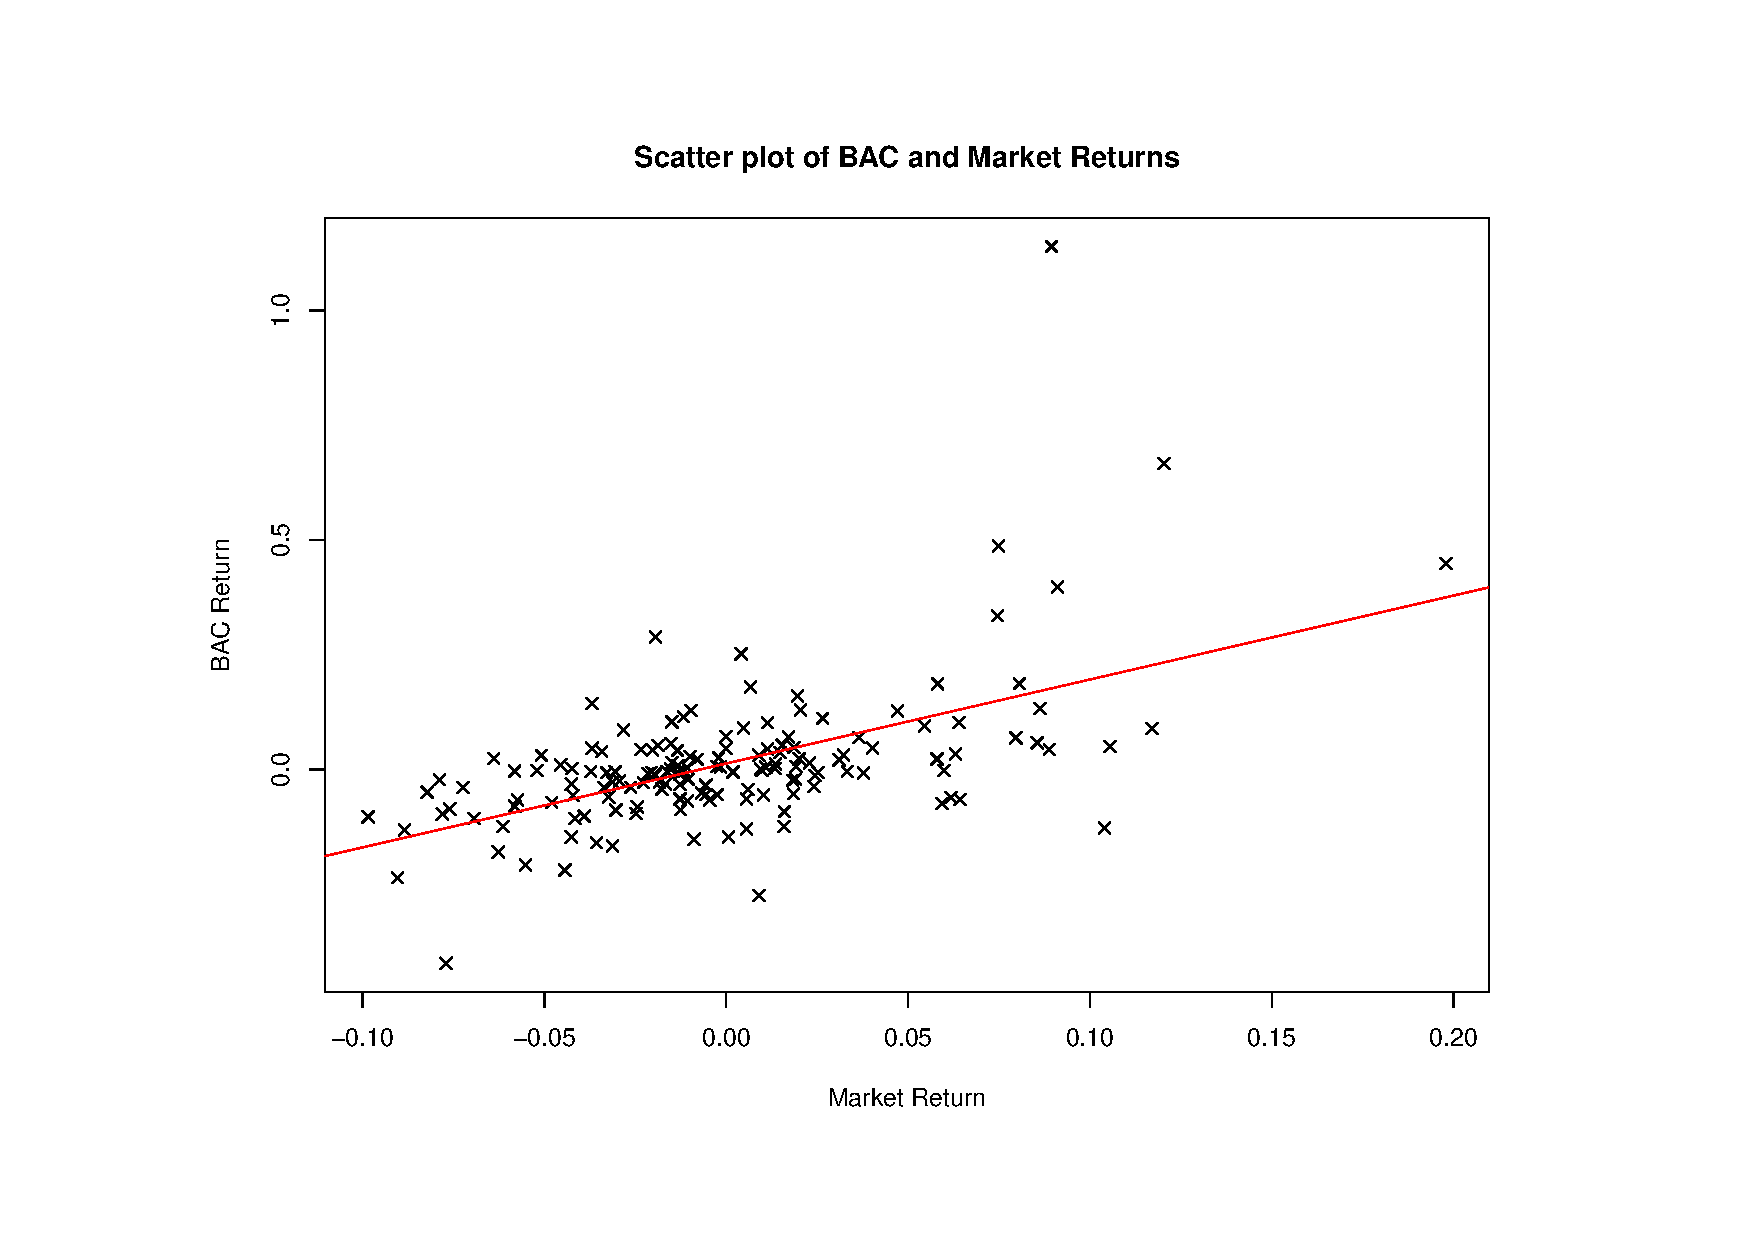
\includegraphics[height = 3.2in]{BACeq}
\end{center}
\end{frame} 

\begin{frame}{Solution 1}
$ y_t = a + bx_t + u_t$
\vskip 1cm
Minimise the residuals
\begin{align*}
Min\sum_{t=1}^{t=T}& u_t^2 \\
Min\sum_{t=1}^{t=T}& (y_t - a - bx_t)^2 
\end{align*}
Take, partial derivative to get the condictions.
\end{frame}

\begin{frame}{Solution 2}
\begin{align*}
\frac{\delta u}{\delta a} = \sum_{t=1}^{t=T} 2(y_t - a - bX_t) =& 0\\
\frac{\delta u}{\delta b} = \sum_{t=1}^{t=T} 2X_t(y_t - a - bx_t) =& 0
\end{align*}
Re-arrange
\begin{align*}
\hat{b} =& \frac{\sum x \sum y - \frac{\sum x \sum y}{T}}{\sum x^2 - \frac{(\sum x)^2}{T}}\\
\hat{a} = & \bar{Y} - b\bar{X}
\end{align*}
\end{frame}

\begin{frame}{Solution: matrix form}
In matrix form
\begin{align*}
\mathbf{y} =& \mathbf{X \beta} + \mathbf{u}\\
\mathbf{u} =& \mathbf{y} - \mathbf{X\beta}\\
\mathbf{u}` \mathbf{u} =& (\mathbf{X \beta} + \mathbf{u})`(\mathbf{X \beta} + \mathbf{u})\\ 
\end{align*}
Taking derivative and re-arranging (see textbook for proof)
\begin{align*}
\mathbf{\beta} = \mathbf{(X`X)}^{-1}\mathbf{X`y}
\end{align*}
\end{frame}

\begin{frame}{Regression Table}
% latex table generated in R 3.0.2 by xtable 1.7-1 package
% Wed Dec 25 22:07:07 2013
\begin{table}[ht]
\rowcolors{1}{OliveGreen!20}{OliveGreen!5}
\centering
\begin{tabular}{rrrrr}
  \hline
 & Estimate & Std. Error & t value & Pr($>$$|$t$|$) \\ 
  \hline
(Intercept) & 0.0130 & 0.0105 & 1.23 & 0.2203 \\ 
  SPY.R & 1.8303 & 0.2240 & 8.17 & 0.0000 \\ 
   \hline
\end{tabular}
\end{table}
The Adjusted $R^2$ is 0.29, therefore nearly 30\% of the BAC returns are explained by the returns of the market.  95\% confidence intervals for the $\beta$ are 1.39 to 2.27. 
\end{frame}


\begin{frame}{Ordinary Least Squares (OLS)}
There are two important qualities that are desiable in an \emph{estimator}
\begin{itemize}[<+-| alert@+>]
\item Unbiased:  the expected value of the estimator is equal to the population value
\item Efficient: Estimates should be as close as possible to the true value 
\end{itemize}
\pause
Given a number of assumptions OLS is the BLUE \textbf{B}est, \textbf{L}inear, \textbf{U}nbiased, \textbf{E}stimator.   
\end{frame}

\section{OLS Assumptions}
\begin{frame}{OLS Assumptions}
The assumptions for BLUE OLS qualities
\pause
\begin{itemize}[<+-| alert@+>]
\item The errors have a zero mean
\item The errors are \emph{independent and identically distributed} (iid)
\begin{itemize}
\item No serial correlation (errors related to each other)
\item Hetroskedasticity (some errors are systematically larger than others)
\end{itemize}
\item Explanatory variables are not related to the error
\item Additionally, assume \emph{normal errors} if we want to use normal assumption to compute \emph{t-tests} of coefficients
\end{itemize}
\end{frame}

\begin{frame}{Issues}
Therefore, there are a number of potential problems
\begin{itemize}[<+-| alert@+>]
\item Functional form
\begin{itemize}
\item Linear form
\item Missing or superfluous variables
\item Structural breaks
\end{itemize}
\item Evidence of problems
\begin{itemize}
\item Serial correlation in the residuals
\item Hetroscedasticity in the residuals
\end{itemize}
\end{itemize}
\end{frame}

\section{Identifying and dealing with problems}
\begin{frame}{Model Problems: Missing Variables}
If explanatory variables are missing
\pause
\begin{itemize}[<+-| alert@+>]
\item Does theory suggest other variables are important?
\item Tests of structural form and residuals will indicate problems
\item Estimates of coefficients will be biased if there is a relationship between estimated and missing variables
\item Estimated errors will be too large or too small
\end{itemize}
\pause
\begin{block}{}
Solution:
Add missing variable or a proxy
\end{block}
\end{frame}

\begin{frame}{Model Problems: Superfluous Variables}
Unnecessary variables
\pause
\begin{itemize}[<+-| alert@+>]
\item Theory and the t-statistic should guide
\item Estimates are unbiased but inefficient.
\item Multicolinearity is a problem
\begin{itemize}
\item Measuring the same thing twice
\item Singular matrix
\end{itemize}
\end{itemize}
\pause
\begin{block}{}
Solution:
Remove superfluous variable.  Be careful of \emph{the dummy variable problem}
\end{block}
\end{frame}

\begin{frame}{Appropriate model}
There are two additional issues to be aware of 
\pause
\begin{itemize}[<+-| alert@+>]
\item Linear model
\begin{itemize}
\item Non-linear relationship
\item Can variables be transformed (logs)
\end{itemize}
\item Structural breaks
\begin{itemize}
\item Shifts in parameters
\item Use dummy variables
\end{itemize}
\end{itemize}
\end{frame}


\section{Further Reading}
\begin{frame}{Eviews}
\begin{itemize}[<+-| alert@+>]
\item \href{http://www.eviews.com/home.html}{Eviews Website}
\item \href{http://www.eviews.com/Learning/index.html}{Tutorials}
\item User Guide 1 Chapter 11 (p. 315 to 321)
\item User Guide 2 Chapter 18 (p. 1 to 22 )
\end{itemize}
\end{frame}

\begin{frame}{Textbooks}
All in the library
\pause
\begin{itemize}[<+-| alert@+>]
\item C. Dougherty, "Introduction to Econometrics", OUP
\item JH Stock and M Watson "Introduction to Econometrics",  Pearson
\item D Gujarati, "Basic Econometrics", McGraw-Hill
\end{itemize}  
\end{frame}



\begin{frame}{Bibliography}
\bibliography{myref}
\end{frame}
\end{document}
